% Options for packages loaded elsewhere
\PassOptionsToPackage{unicode}{hyperref}
\PassOptionsToPackage{hyphens}{url}
\PassOptionsToPackage{dvipsnames,svgnames,x11names}{xcolor}
%
\documentclass[
  letterpaper,
  DIV=11,
  numbers=noendperiod]{scrartcl}

\usepackage{amsmath,amssymb}
\usepackage{iftex}
\ifPDFTeX
  \usepackage[T1]{fontenc}
  \usepackage[utf8]{inputenc}
  \usepackage{textcomp} % provide euro and other symbols
\else % if luatex or xetex
  \usepackage{unicode-math}
  \defaultfontfeatures{Scale=MatchLowercase}
  \defaultfontfeatures[\rmfamily]{Ligatures=TeX,Scale=1}
\fi
\usepackage{lmodern}
\ifPDFTeX\else  
    % xetex/luatex font selection
\fi
% Use upquote if available, for straight quotes in verbatim environments
\IfFileExists{upquote.sty}{\usepackage{upquote}}{}
\IfFileExists{microtype.sty}{% use microtype if available
  \usepackage[]{microtype}
  \UseMicrotypeSet[protrusion]{basicmath} % disable protrusion for tt fonts
}{}
\makeatletter
\@ifundefined{KOMAClassName}{% if non-KOMA class
  \IfFileExists{parskip.sty}{%
    \usepackage{parskip}
  }{% else
    \setlength{\parindent}{0pt}
    \setlength{\parskip}{6pt plus 2pt minus 1pt}}
}{% if KOMA class
  \KOMAoptions{parskip=half}}
\makeatother
\usepackage{xcolor}
\setlength{\emergencystretch}{3em} % prevent overfull lines
\setcounter{secnumdepth}{-\maxdimen} % remove section numbering
% Make \paragraph and \subparagraph free-standing
\makeatletter
\ifx\paragraph\undefined\else
  \let\oldparagraph\paragraph
  \renewcommand{\paragraph}{
    \@ifstar
      \xxxParagraphStar
      \xxxParagraphNoStar
  }
  \newcommand{\xxxParagraphStar}[1]{\oldparagraph*{#1}\mbox{}}
  \newcommand{\xxxParagraphNoStar}[1]{\oldparagraph{#1}\mbox{}}
\fi
\ifx\subparagraph\undefined\else
  \let\oldsubparagraph\subparagraph
  \renewcommand{\subparagraph}{
    \@ifstar
      \xxxSubParagraphStar
      \xxxSubParagraphNoStar
  }
  \newcommand{\xxxSubParagraphStar}[1]{\oldsubparagraph*{#1}\mbox{}}
  \newcommand{\xxxSubParagraphNoStar}[1]{\oldsubparagraph{#1}\mbox{}}
\fi
\makeatother


\providecommand{\tightlist}{%
  \setlength{\itemsep}{0pt}\setlength{\parskip}{0pt}}\usepackage{longtable,booktabs,array}
\usepackage{calc} % for calculating minipage widths
% Correct order of tables after \paragraph or \subparagraph
\usepackage{etoolbox}
\makeatletter
\patchcmd\longtable{\par}{\if@noskipsec\mbox{}\fi\par}{}{}
\makeatother
% Allow footnotes in longtable head/foot
\IfFileExists{footnotehyper.sty}{\usepackage{footnotehyper}}{\usepackage{footnote}}
\makesavenoteenv{longtable}
\usepackage{graphicx}
\makeatletter
\def\maxwidth{\ifdim\Gin@nat@width>\linewidth\linewidth\else\Gin@nat@width\fi}
\def\maxheight{\ifdim\Gin@nat@height>\textheight\textheight\else\Gin@nat@height\fi}
\makeatother
% Scale images if necessary, so that they will not overflow the page
% margins by default, and it is still possible to overwrite the defaults
% using explicit options in \includegraphics[width, height, ...]{}
\setkeys{Gin}{width=\maxwidth,height=\maxheight,keepaspectratio}
% Set default figure placement to htbp
\makeatletter
\def\fps@figure{htbp}
\makeatother

\KOMAoption{captions}{tableheading}
\makeatletter
\@ifpackageloaded{caption}{}{\usepackage{caption}}
\AtBeginDocument{%
\ifdefined\contentsname
  \renewcommand*\contentsname{Table of contents}
\else
  \newcommand\contentsname{Table of contents}
\fi
\ifdefined\listfigurename
  \renewcommand*\listfigurename{List of Figures}
\else
  \newcommand\listfigurename{List of Figures}
\fi
\ifdefined\listtablename
  \renewcommand*\listtablename{List of Tables}
\else
  \newcommand\listtablename{List of Tables}
\fi
\ifdefined\figurename
  \renewcommand*\figurename{Figure}
\else
  \newcommand\figurename{Figure}
\fi
\ifdefined\tablename
  \renewcommand*\tablename{Table}
\else
  \newcommand\tablename{Table}
\fi
}
\@ifpackageloaded{float}{}{\usepackage{float}}
\floatstyle{ruled}
\@ifundefined{c@chapter}{\newfloat{codelisting}{h}{lop}}{\newfloat{codelisting}{h}{lop}[chapter]}
\floatname{codelisting}{Listing}
\newcommand*\listoflistings{\listof{codelisting}{List of Listings}}
\makeatother
\makeatletter
\makeatother
\makeatletter
\@ifpackageloaded{caption}{}{\usepackage{caption}}
\@ifpackageloaded{subcaption}{}{\usepackage{subcaption}}
\makeatother

\ifLuaTeX
  \usepackage{selnolig}  % disable illegal ligatures
\fi
\usepackage{bookmark}

\IfFileExists{xurl.sty}{\usepackage{xurl}}{} % add URL line breaks if available
\urlstyle{same} % disable monospaced font for URLs
\hypersetup{
  colorlinks=true,
  linkcolor={blue},
  filecolor={Maroon},
  citecolor={Blue},
  urlcolor={Blue},
  pdfcreator={LaTeX via pandoc}}


\author{}
\date{}

\begin{document}


\section{Cultures of Listening}\label{cultures-of-listening}

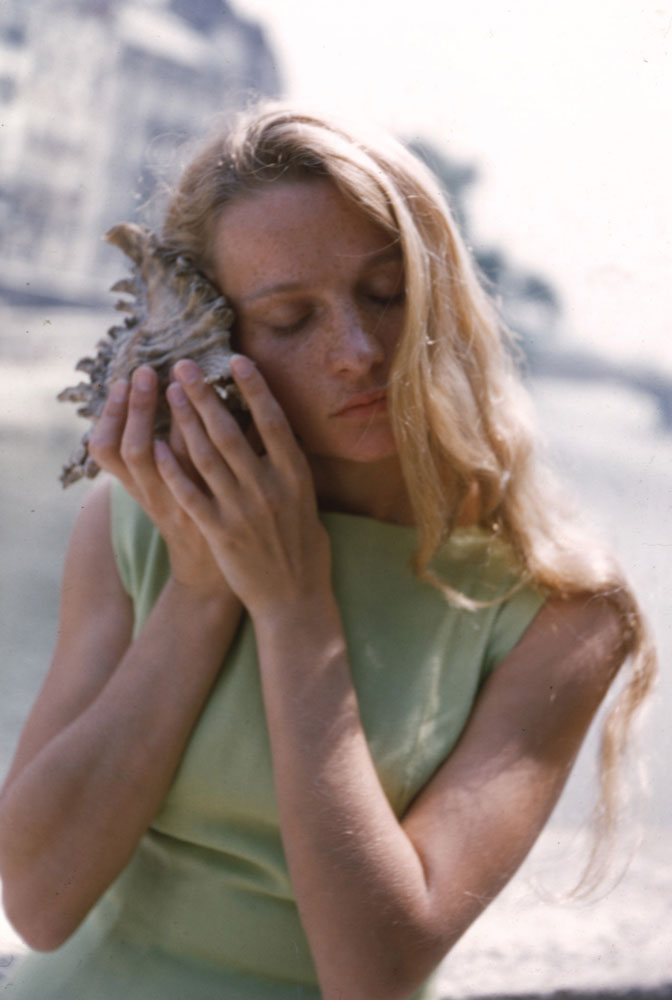
\includegraphics[width=0.4\textwidth,height=\textheight]{eliane-radigue.jpg}

Cheshire Academy for Lifelong Learning (CALL)\\
Keene State College\\
Spring Semester 2018\\
Instructor: Dr.~Martin Roberts\\
Class: Friday 10:00-11:15 a.m.\\
Location: Morrison Hall 109\\
\href{mailto:dokoissho@pm.me}{dokoissho@sdf.org}\\

\subsection{Overview}\label{overview}

How do we listen to music today? How is that different from how people
listened to it a decade ago? A generation ago? A century ago? Why listen
to music at all? This course provides an introduction to how to listen
to music, and sound more generally, in a digital age of playlists and
short attention spans. Rather than a traditional music-appreciation
course, however, it focuses on listening itself as a cultural practice
of the modern age. Topics include easy listening, hi-fi, and stereo in
1950s suburbia; jukeboxes and the rise of popular music; multitrack
recording and headphone music in the 60s; portable listening from the
Sony Walkman to the Apple iPod; elevator music, and ubiquitous
listening; field recording and acoustic ecology; audiophile culture and
the vinyl revival; streaming media and the playlist. Each class will be
structured around relevant reading materials and a collective listening
session and discussion. The course's objective is to develop an
understanding of listening as a deeply cultural practice, and to teach
us to listen more attentively to the sounds of the world around us.

\subsection{Instructor Bio}\label{instructor-bio}

Dr.~Martin Roberts holds a Ph. D. in French Studies from Cambridge
University. He has taught at Harvard University, MIT, The New School,
and NYU, and is currently Visiting Professor in the Department of Film
and Media Studies at Dartmouth College. He has published essays on world
music, and his courses on music include Music as Communication~and
BeatleMedia: Popular Music and Cultural Heritage.

\subsection{Reading Assignments}\label{reading-assignments}

Readings are either available online or as PDF files for download and
printing: see links below.

\subsection{Recommended Reading}\label{recommended-reading}

John Himmelman, \textbf{Cricket Radio: Tuning In the Night-Singing
Insects.} Cambridge: Harvard University Press, 2011.

Damon Krukowski, \textbf{The New Analog: Listening and Reconnecting in a
Digital World.} New York: The New Press, 2017.

Joseph Lanza, \textbf{Elevator Music: A Surreal History of Muzak,®
Easy-Listening, and Other Moodsong.} Revised and expanded edition. Ann
Arbor: University of Michigan Press, 2004.

Pauline Oliveros, \textbf{Deep Listening: A Composer's Sound Practice.}
Lincoln, NE: Deep Listening Publications, 2005.

Ben Ratliff, \textbf{Every Song Ever: Twenty Ways to Listen to Music
Now.} London: Penguin Books, 2016.

R. Murray Schafer, \textbf{The Soundscape: Our Sonic Environment and the
Tuning of the World.} Rochester, VT: Destiny Books, 1994. Originally
published as \textbf{The Tuning of the World.} New York: Alfred A.
Knopf, 1997.

Paul Théberge, Kyle Devine, and Tom Everrett, eds., \textbf{Living
Stereo: Histories and Cultures of Multichannel Sound.} New York:
Bloomsbury, 2015.

David Toop, \textbf{Ocean of Sound: Aether Talk, Ambient Sound and
Imaginary Worlds.} London: Serpent's Tail, 1995.

\subsection{Other Resources}\label{other-resources}

\href{https://www.google.com/url?q=http://www.youtube.com/watch?v\%3DfYp6NhwIkjU&sa=D&ust=1600611913237000&usg=AOvVaw33MX-ZmRoea0Dq8zmhmaCX}{Class
YouTube playlist}

\subsection{Course Schedule}\label{course-schedule}

\begin{longtable}[]{@{}
  >{\raggedright\arraybackslash}p{(\columnwidth - 4\tabcolsep) * \real{0.0536}}
  >{\raggedright\arraybackslash}p{(\columnwidth - 4\tabcolsep) * \real{0.9324}}
  >{\raggedright\arraybackslash}p{(\columnwidth - 4\tabcolsep) * \real{0.0117}}@{}}
\toprule\noalign{}
\endhead
\bottomrule\noalign{}
\endlastfoot
Week & Topic & \\
1: Fri 9 March 2018 &
\multicolumn{2}{>{\raggedright\arraybackslash}p{(\columnwidth - 4\tabcolsep) * \real{0.9441} + 2\tabcolsep}@{}}{%
\textbf{Field Recordings} \textbar{} \textbar{} John Himmelman,
\href{https://www.google.com/url?q=http://www.cricketradiobroadcast.com/&sa=D&ust=1600611913239000&usg=AOvVaw1k6hnm-J-fsfbt9LGHxIqK}{Cricket
Radio} \textbar{} \textbar{} Lafcadio Hearn,
``\href{https://www.google.com/url?q=http://www.bolingo.org/cricket/galleries/hearn2/source/157_frogs.htm&sa=D&ust=1600611913239000&usg=AOvVaw1f1Tz5Ryx5nFU0pcd_AwRo}{Frogs}''
(\textbf{Exotics and Retrospectives}, 1898). \textbar{} \textbar{}
\href{https://www.google.com/url?q=http://www.orca-live.net/&sa=D&ust=1600611913240000&usg=AOvVaw1hPNXiwI6jgNplE_mF4qnd}{Orca.fm}
\textbar{} \textbar{} Steven Feld, Voices of the Rainforest \textbar{}
\textbar{}
\href{https://www.google.com/url?q=http://www.bolingo.org/cricket/galleries/hearn2/source/157_frogs.htm&sa=D&ust=1600611913240000&usg=AOvVaw3GaWl1UfoD8K3GUVvkpV_m}{Suikinkutsu
article} \textbar{} \textbar{}
\href{https://www.google.com/url?q=https://quietamerican.org/introduction.html&sa=D&ust=1600611913241000&usg=AOvVaw01D_Ef_TjtcjZ_Y8sJ58D0}{The
Quiet American} \textbar{}} \\
2: Fri 16 March 2018 &
\multicolumn{2}{>{\raggedright\arraybackslash}p{(\columnwidth - 4\tabcolsep) * \real{0.9441} + 2\tabcolsep}@{}}{%
\textbf{Deep Listening: Soundscapes \& Acoustic Ecology} \textbar{}
\textbar{} Read: \textbar{} \textbar{} Kerry O'Brien,
``\href{https://www.google.com/url?q=https://www.newyorker.com/culture/culture-desk/listening-as-activism-the-sonic-meditations-of-pauline-oliveros&sa=D&ust=1600611913242000&usg=AOvVaw0CdCElBgTFgn5ps4H4xg2P}{Listening
as Activism: The `Sonic Meditations' of Pauline Oliveros}'' (New Yorker)
\textbar{} \textbar{} Murray Schafer,
\href{https://www.google.com/url?q=https://drive.google.com/file/d/1FV0Z0w89ucQ_wXMNM9qMLLBezGHzaPVn/view?usp\%3Dsharing&sa=D&ust=1600611913242000&usg=AOvVaw15KbOLoy5RG5ALmhgwtMHW}{Introduction
to}
\href{https://www.google.com/url?q=https://drive.google.com/file/d/1FV0Z0w89ucQ_wXMNM9qMLLBezGHzaPVn/view?usp\%3Dsharing&sa=D&ust=1600611913243000&usg=AOvVaw1YZcp9ng2MQa_9N3SrLUn0}{\textbf{The
Soundscape}} \textbar{} Kendall Wrightson,
``\href{https://www.google.com/url?q=https://drive.google.com/file/d/1QfBuhibIeXYXsDfnwJ8krgS7k6JNA0Zj/view?usp\%3Dsharing&sa=D&ust=1600611913243000&usg=AOvVaw1OszPqBYF9UjI9roC7CWmn}{An
Introduction to Acoustic Ecology}'' \textbar{} \textbar{} Listen:
\textbar{} \textbar{} Deep Listening Band, \textbf{The Ready Made
Boomerang} \textbar{}} \\
3: Fri 23 March 2018 &
\multicolumn{2}{>{\raggedright\arraybackslash}p{(\columnwidth - 4\tabcolsep) * \real{0.9441} + 2\tabcolsep}@{}}{%
\textbf{Background Music: Easy Listening and Muzak} \textbar{}
\textbar{} Read: \textbar{} \textbar{} Keir Keightley,
``\href{https://www.google.com/url?q=https://drive.google.com/file/d/15K7Yf0776mxoUMN7FlXGc8IJHuYKHCEV/view?usp\%3Dsharing&sa=D&ust=1600611913245000&usg=AOvVaw3DyAwXEbJRMCNTkuN8Vh98}{Music
for Middlebrows: Defining the Easy Listening Era, 1946-66}'' \textbar{}
\textbar{} Tim Anderson, ``Training the Listener: Stereo Demonstration
Disks in an Emerging Consumer Market'' \textbar{} \textbar{} Joseph
Lanza, selected chs.~from \textbf{Elevator Music} \textbar{} \textbar{}
Listen: \textbar{} \textbar{} \textbf{Audio Fidelity Stereo Spectacular
Demonstration and Sound Effects} (1962) \textbar{}} \\
4: Fri 30 March 2018 &
\multicolumn{2}{>{\raggedright\arraybackslash}p{(\columnwidth - 4\tabcolsep) * \real{0.9441} + 2\tabcolsep}@{}}{%
\textbf{Strange Sounds: Electronic Listening} \textbar{} \textbar{}
Watch/listen: \textbar{} \textbar{}
\href{https://www.google.com/url?q=https://vimeo.com/215437182&sa=D&ust=1600611913246000&usg=AOvVaw2ncqxBscCnzABqDHMati9z}{\textbf{The
Delian Mode}}~(documentary about Delia Derbyshire) \textbar{} \textbar{}
``\href{https://www.google.com/url?q=http://www.bbc.co.uk/programmes/b00rl2ky&sa=D&ust=1600611913247000&usg=AOvVaw3rv1pbI9kBWVfiOGmgSGp9}{\textbf{Sculptress
of Sound: The Lost Works of Delia Derbyshire}}'' (BBC Radio 4, 29 March
2010) \textbar{} \textbar{}
\href{https://www.google.com/url?q=https://vimeo.com/87398243&sa=D&ust=1600611913247000&usg=AOvVaw0LvVFQwUV-LT1Z6APF7dNb}{\textbf{IMA
fiction \#4: Eliane Radigue}} (15-min. video) \textbar{} \textbar{}
In-class: excerpt from
\href{https://www.google.com/url?q=https://scottdoc.com/&sa=D&ust=1600611913248000&usg=AOvVaw03EVoIN158ukV0mvFYiz7R}{\textbf{Deconstructing
Dad}}~(documentary about Raymond Scott) \textbar{}} \\
5: Fri 6 April 2018 &
\multicolumn{2}{>{\raggedright\arraybackslash}p{(\columnwidth - 4\tabcolsep) * \real{0.9441} + 2\tabcolsep}@{}}{%
\textbf{Music for Airports: Ubiquitous Listening} \textbar{} \textbar{}
Read: \textbar{} \textbar{} Geeta Dayal excerpt from \textbf{Another
Green World} \textbar{} \textbar{} Listen: \textbar{} \textbar{} Brian
Eno, \textbf{Music For Airports} \textbar{} \textbar{} Jake Tilson,
\textbf{Gate 63} (in class) \textbar{} \textbar{} Easy Jet,
\href{https://www.google.com/url?q=https://www.youtube.com/watch?v\%3DmLwrmJFUa4Q\%26index\%3D2\%26list\%3DPLKJL7wxYKW3Mkiaj-ql1H9V21kq48NMGn\%26t\%3D0s&sa=D&ust=1600611913250000&usg=AOvVaw02QJ1GTUI4iEzP0gORFSZX}{Jet
Sounds}
(\href{https://www.google.com/url?q=https://itunes.apple.com/tr/album/jet-sounds/1271544738&sa=D&ust=1600611913250000&usg=AOvVaw0OwJm-yAHdyhrChFx_FE4T}{iTunes})
\textbar{}} \\
6: Fri 13 April 2018 &
\multicolumn{2}{>{\raggedright\arraybackslash}p{(\columnwidth - 4\tabcolsep) * \real{0.9441} + 2\tabcolsep}@{}}{%
\textbf{Listening In: Eavesdropping} \textbar{} \textbar{} Scanner
(Robin Rimbaud): various recordings tba \textbar{} \textbar{}
\textbf{The Ghost Orchid} (EVP compilation) \textbar{}} \\
7: Fri 20 April 2018 &
\multicolumn{2}{>{\raggedright\arraybackslash}p{(\columnwidth - 4\tabcolsep) * \real{0.9441} + 2\tabcolsep}@{}}{%
\textbf{Headspace: Listening over Headphones} \textbar{} \textbar{}
Read: \textbar{} \textbar{} Damon Krukowski, ``Headspace'' (in
\textbf{The New Analog}) \textbar{} \textbar{} Shuhei Hosokawa, ``The
Walkman Effect'' \textbar{} \textbar{} Michael Bull, ``Investigating the
Culture of Mobile Listening'' \textbar{} \textbar{} Listen: Pink Floyd,
\textbf{The Dark Side of the Moon} \textbar{}} \\
8: Fri 27 April 2017 &
\multicolumn{2}{>{\raggedright\arraybackslash}p{(\columnwidth - 4\tabcolsep) * \real{0.9441} + 2\tabcolsep}@{}}{%
\textbf{Analog Listening in the Digital Age} \textbar{} \textbar{}
Listen: \textbar{} \textbar{} Damon Krukowski,
\href{https://www.google.com/url?q=https://www.radiotopia.fm/showcase/ways-of-hearing&sa=D&ust=1600611913253000&usg=AOvVaw1QEG3p3FPx24P21_59PL0s}{\textbf{Ways
of Hearing}}~podcast \textbar{} \textbar{} Read: \textbar{} \textbar{}
Janet Borgerson and Jonathan Schroeder, seelcted chs.~from
\textbf{Designed For Hi-Fi Living} \textbar{} \textbar{} Ben Ratlif,
selected chs.~from \textbf{Every Song Ever} \textbar{}} \\
\end{longtable}




\end{document}
